\begin{juliacode}
using Gadfly
x = linspace(0, 2π, 200)
plot(x=x, y = sin(x), Geom.line)
\end{juliacode}
\begin{figure}[ht]
\center
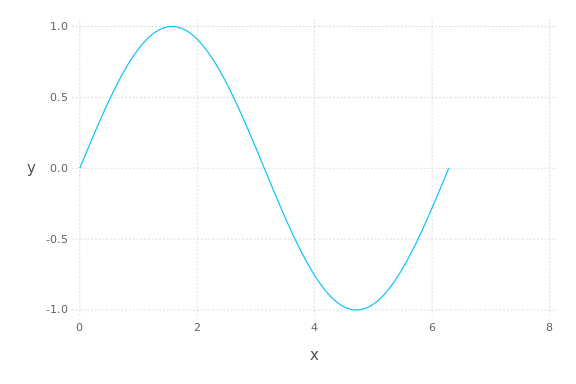
\includegraphics[width=\linewidth]{figures/gadfly_formats_test_sin_fun_1.pdf}
\caption{sin(x) function.}
\label{fig:sin_fun}
\end{figure}

\begin{figure}[htpb]
\center
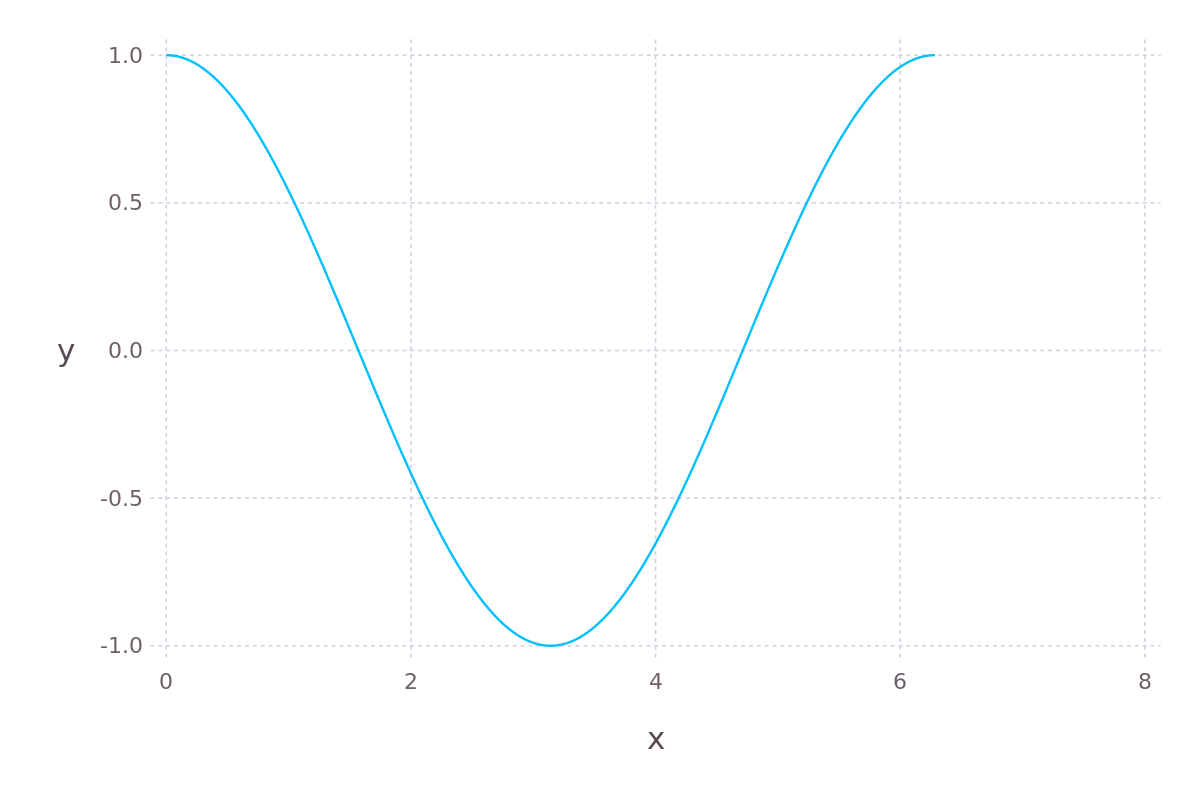
\includegraphics[width=\linewidth]{figures/gadfly_formats_test_2_1.pdf}
\caption{cos(x) function.}
\end{figure}

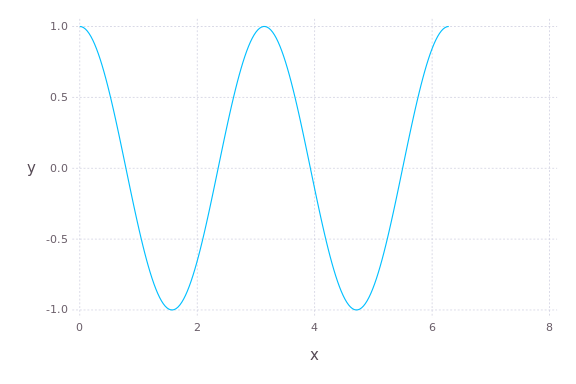
\includegraphics[width=\linewidth]{figures/gadfly_formats_test_cos2_fun_1.pdf}

\begin{juliaterm}
julia> x = linspace(0, 2π, 200)
200-element LinSpace{Float64}:
 0.0,0.0315738,0.0631476,0.0947214,0.126295,…,6.18846,6.22004,6.25161,6.28319

julia> plot(x=x, y = sin(x), Geom.line)

\end{juliaterm}
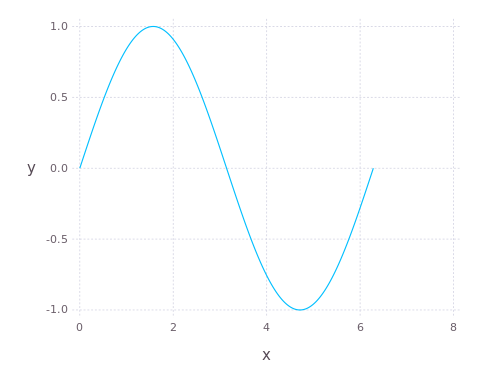
\includegraphics[width=\linewidth]{figures/gadfly_formats_test_4_1.pdf}

\begin{juliaterm}
julia> y = 20
20

julia> plot(x=x, y = cos(x), Geom.line)

\end{juliaterm}
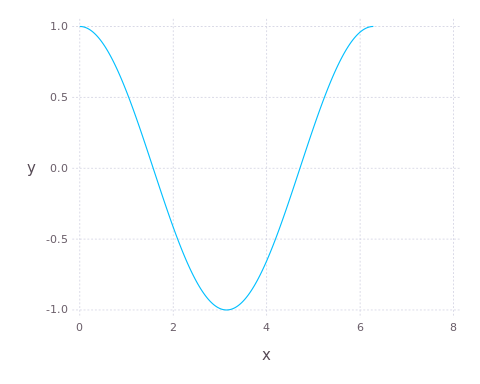
\includegraphics[width=\linewidth]{figures/gadfly_formats_test_4_2.pdf}

\begin{juliacode}
x = linspace(0, 2π, 200)
plot(x=x, y = sin(x), Geom.line)
\end{juliacode}
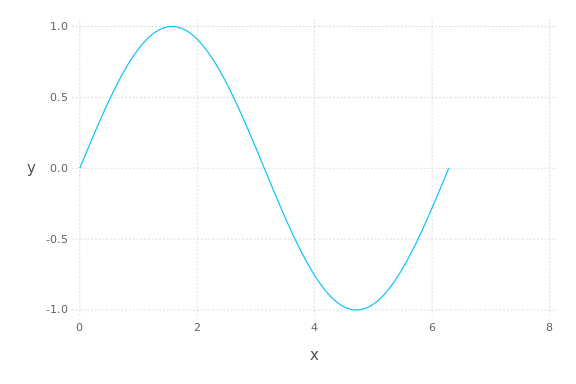
\includegraphics[width=15cm]{figures/gadfly_formats_test_5_1.pdf}

\begin{juliacode}
y = 20
plot(x=x, y = cos(x), Geom.line)
\end{juliacode}
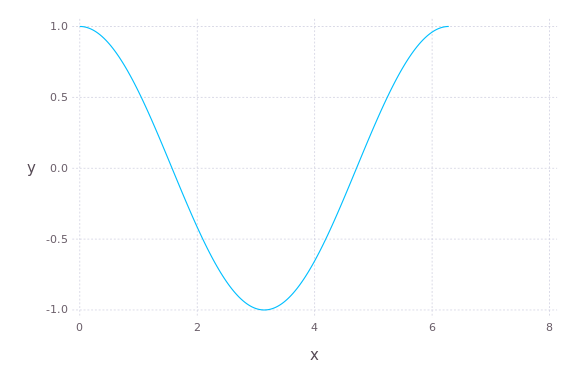
\includegraphics[width=15cm]{figures/gadfly_formats_test_5_2.pdf}
